\documentclass[bibliography=totoc]{scrartcl}

\usepackage[ngerman]{babel}
\usepackage[T1]{fontenc}
\usepackage[utf8]{inputenc}
\usepackage[a4paper]{geometry}
\usepackage{microtype}
\usepackage{amsmath, amssymb, amsfonts, amsopn, mathtools}
\usepackage{hyperref}
\usepackage{appendix}
\usepackage{tabularx}
\usepackage{booktabs}
\usepackage{graphicx}
\usepackage{tikz}
\usepackage{pgfgantt}
\usepackage{float}

\begin{document}
		\title{\vspace{-2cm}Abschlussbericht}
		\subtitle{Named Entity Classification}
		\author{Madita Huvar, Phillip Richter-Pechański, Sanaz Safdel} 
		
		\maketitle
		
		\newpage
		
		\tableofcontents
		
		\newpage
		
\section{Einführung}
	Named Entity Recognition (NER) ist bereits seit den 1990er Jahren ein aktives Forschungsfeld.\cite{Borthwick99}\cite{Tjong2003}\cite{Marrero2013}
	NER bilder die Grundlage für weitere Forschung in vielen Bereichen der maschinellen Sprachverarbeitung, u.a. Information Retrieval, Semantic Annotation, Question Answering, Opinion Mining, usw.\cite{Marrero2013}
	\subsection{Was sind Named Entities?}
		Named Entities sind Phrasen, die Namen von Personen, Organisationen,
		Währungen, Orten usw. enthalten. Eine Named Entity kann abstrakter oder physischer Natur sein. Für weitere Informationen siehe (\url{https://en.wikipedia.org/wiki/Named_entity}).\\
		Im Folgenden sind einige Beispiele für Named Entities aufgelistet:
		\begin{itemize}
			\item The Speaker of the [ORG U.N.] ...
			\item President [PER Obama] ...
			\item The price of the [MONEY Dollar] lost ...
			\item The city of [LOC Moscow] is the capital of Russia.
		\end{itemize}

\section{Unser Projekt}
	Typischerweise werden Named Entity Recognition und Named Entity
	Classification (NEC) zusammen betrachtet. Nur wenige Untersuchungen beschäftigen sich ausschließlich mit NEC.\cite{Primadhanty2014}\cite{He2016} Im Gegensatz zur NER beschäftigt sich die NEC nur mit positiven NE-Instanzen. Dies führt dazu, dass dieses Projekt als globales Evaluationsmaß lediglich Accuracy nutzt, da $Precision=Accuracy$. \footnote{siehe \url{http://www.cl.uni-heidelberg.de/courses/ss16/annotierteKorpora/material/NLPW_SS16_F04_EvalPRFA.pdf}}
	\subsection{Ziel}
	Dieses Projekt konzentriert sich auf NEC und stellt die Frage, \textbf{welchen Einfluss Feature Selection auf die
	Klassifikationsergebnisse eines Named Entity Klassifizierers hat}.
	Dabei nutzen wir einfache syntaktische und lexikalische Features, die bereits in fast allen Forschungsarbeiten in ähnlicher Form genutzt wurden. \cite{Toral2006}\cite{Kazama2007}\cite{Ratinov2009}
	\subsection{Organisation}
	Für unser Projekt haben wir einige nützliche Tools zum kollaborativen Arbeiten genutzt. Für Aufgaben rund ums Thema Programmierung haben wir GitHub (\url{https://github.com/MaviccPRP/ml_ner}) eingesetzt. Zum Austausch organisatorischer Fragen, nutzten wir eine eigene Whatsapp Gruppe. Zwischenergebnisse und Protokolle gemeinsamer Treffen haben wir in einer eigens angelegten Wikiseite festgehalten. \footnote{\url{https://wiki.cl.uni-heidelberg.de/foswiki/bin/view/Studenten/MLGruppeNERRec}}
\section{Daten und Tools}
	Unser Projekt baute im Wesentlichen  auf folgende Tools auf:
				\begin{itemize}
					\item Python 3.4+
					\item Scikit Learn als Klassifizierer
					\item liac-arff
					\item matplotlib
					\item Weka zur Korpusanalyse
				\end{itemize}
		Python 3 kommt zum Einsatz, weil diese Version eine problemlose Verarbeitung von Unicode ermöglicht. Der Scikit Learn Klassifizierer bietet gute Evaluationstools, die in diesem Projekt zum Einsatz gekommen sind. Das Modul liac-arff wandelt Python Dictionaries in .arff-Dateien um, wodurch wir mittels WEKA Korpusanalysen durchführen konnten.
	\subsection{Korpus}
	Für die Named Entity Klassifikation wurde der OntoNotes Korpus 2012 genutzt.\cite{Weischedel2013}
	Wir konzentrierten uns dabei lediglich auf die englischen Nachrichtentexte des ’The Wall Street Journal’. Für unsere
	Entwicklungsphase stellte der Korpus ein bereits vorgefertigtes Developmentset zu Verfügung. Für die eigentliche Klassifikation der Named Entities kamen dann die Trainings- und Testdatensets des Korpus zum Einsatz. Während das Trainingsset den manuell annotierten Goldstandard enthielt, griffen wir beim Testset auf die automatisch annotierten Datensets des OntoNotes Korpus zurück, da kein Goldstandard zur Verfügung stand. Die Anzahl der Named Entity Instanzen in den verschiedenen Datensets sind in Tabelle \ref{tab:corpus} zusammengefasst.
	\subsection{Korpusreader}
	Für die Extraktion der Named Entities wurde ein Korpusreader erstellt. Der Reader extrahiert alle Named Entities und weist ihnen folgende Informationen zu.
	
	\begin{itemize}
		\item POS-Tags der einzelnen Token
		\item Phrasenart der Instanz
		\item Kontextwörter (ne-1, ne+1) der Instanz
		\item Instanzklasse
	\end{itemize}
	Im Folgenden eine Beispielextraktion zu dem Satz:\\
	\textit{Says \textbf{Peter Mokaba}, President of the South African Youth Congress:}\\
	
	\textbf{\{'PERSON':[['Peter', 'NNP'],['Mokaba', 'NNP'],'NP', ('Says', ',')]\}}
	\subsection{Korpusklassen}
	Die verwendeten Korpusklassen im originalen OntoNotes Korpus sind in Tabelle \ref{tab:classesunbalanced} aufgelistet.\\
	Zehn Klassen enthalten dabei nur relativ wenige Named Entity Instanzen. Deshalb haben wir die Klassen für unser Projekt teilweise zusammengefasst. Selten vorkommende Klassen wurden aus dem balancierten Korpus entfernt. Neben semantisch ähnliche Klassen wie NORP und GPE wurden zudem numerische Klassen wie MONEY, PERCENT und CARDINAL zusammengefasst. Eine Beschreibung der Klassen findet sich in Tabelle \ref{tab:descclasses}. Die Anzahl der Named Entity Instanzen sind in Tabelle \ref{tab:countclasses} aufgelistet.
\section{Klassifizierung}
	
	\subsection{Featureset}
	Um eine Art untere Grenze für die Evaluationsergebnisse unseres Klassifizierers zu setzen, wurde eine Baseline definiert. Diese enthielt lediglich Unigramme als Features. Die Unigramme haben wir zuvor nach folgenden Kriterien aus dem Korpus extrahiert:
	\begin{itemize}
		\item Die Unigramme sind Teil einer Named Entity Instanz
		\item Die Unigramme kamen mindestens fünfmal im gesamten Trainingskorpus vor.
	\end{itemize}
	Weitere Details zur Unigrambaseline finden sich in Tabelle \ref{tab:baseline}. Insgesamt produzierte die Baseline 1317 verschiedene Unigramme. Zur besseren Unterscheidung nutzen wir im Folgenden den Begriff Featurekategorie, wenn wir von einem Featuretyp sprechen, wie etwa 'Unigram' und 'POS Tags'. Features sind die atomaren Teile der Featurekategorien. Während die Featurekategorie 'Unigram' über 1300 Features enthält, steht die Featurekategorie 'isInWiki' für lediglich ein Feature.\\
	
	Unser komplettes Featureset, inklusive Beschreibung und Beispielextraktionen, ist in Tabelle \ref{tab:featureset} zusammengefasst. Dabei haben wir drei mehrdimensionale Featurekategorien genutzt. Neben den Unigrammen nutzten wir den Instanzcontext, der jeweils das Token vor und nach der Named Entity Instanz enhält. Darüber hinaus definierten wir noch die Anzahl der verschiedenen POS Tags in den Instanzen.\\
	Insgesamt bestand das komplette Featureset aus 1716 atomaren Features.  
	\subsection{Klassifizierertyp}
	Zur Klassifizierung der Named Entities wurde eine Support Vector Maschine mit
	linearem Kernel verwendet. Nach einer ausführlichen Evaluation\footnote{Zum Tuning der Hyperparameter  kam das Scikit Learn Tool GridSearch zum Einsatz: \url{http://scikit-learn.org/stable/modules/grid_search.html}} aller möglichen Hyperparameter haben sich folgende Einstellungen als optimal erwiesen.
	\begin{itemize}
		\item Klassifiziererklasse='sklearn.svm.LinearSVC'
		\item loss=’squared hinge’
		\item penalty=’l2’
	\end{itemize}

	Unsere Featurevektoren haben sehr viele atomare Features, weshalb der linearer Kernel die besten Ergebnisse lieferte. Bei nichtlinearen Kerneln scheint es zum Overfitting zu kommen. Zudem hat Chih-Wei\cite{Chin-wei2003} festgestellt, dass das Mapping in einen höheren Featurespace eines nicht-linearen Kernels kaum Klassifizierungsverbesserungen gibt.\\
	
	Alternativ wurde ein Decisiontree getestet, dieser hatte allerdings mit
	allen Featurekombinationen tendenziell schlechtere Evaluationsergebnisse. Zudem trainierte die SVM deutlich schneller.
\section{Evaluation}
	Insgesamt wurden elf Featurekategorien eingesetzt. Um die Performance der einzelnen Featurekategorien zu testen, wurde zuerst die Potenzmenge des Featuresets gebildet.
	
	Für die Evaluation entscheidend waren alle Teilmengen, die die Featurekategorien 'Unigram' und 'Context' enthielten und insgesamt mind. drei Featurekategorien besitzen. Diese Einschränkungen wurden zum einen aufgrund von Zeitersparnissen gewählt, außerdem ergaben Tests, dass Klassifizierer ohne diese Mindestanforderungen erheblich schlechtere Ergebnisse lieferten:
				
	\begin{itemize}
	\item Accuracy aller Teilmengen ohne die Featurekategorien 'Unigram' und 'Context': \textless 69\%.
	\item Accuracy nur mit 'Unigram' und 'Context': 87.42\%
	\end{itemize}
				
	Schließlich wurde der Klassifizierer auf allen restlichen 1013 Teilmengen
	durchgeführt. Die Accuracy der einzelnen Klassifizierungen sind in Abbildung \ref{tab:accuracy} dargestellt.\\
	Die höchste Accuracy erreichten wir ab sieben Featurekategorien. Ab vier Featurekategorien gab es kaum mehr Verbesserungen der Accuracywerte. Featurekategorien, die zur Erhöhung der Accuracy beitragen waren insbesondere:
	\begin{itemize}
		\item ’POS’
		\item ’is all caps’
		\item ’is in wiki’
		\item ’is np’
		\item ’contains digit’
	\end{itemize}
	
	Das Featureset bestehend aus den vier Featurekategorien: \textbf{’Unigram’, ’Context’, ’POS’, ’is all caps’} erreichte die beste Accuracy bei möglichts kleinem Featureset.\\
	Die ROC Kurve \ref{tab:roc} und die Confusionmatrix \ref{tab:confusion} geben weitere Auskunft über die Qualität der Klassifizierung. Auffallend ist hier das schlechte Abschneiden der PERSONEN Instanzen. Insbesondere die Precision fällt hier deutlich ab. Mögliche Ursache könnten sein, das wir auch nach der Klassenzusammenfassung, relativ wenige PERSONEN Instanzen im Trainingsset hatten.\\
	
	Tabelle \ref{tab:result} fasst die Evaluationsergebnisse der Baseline im Vergleich zum  optimalem Featureset zusammen. Hierbei wird deutlich, dass sich die Accuracy sowohl der balancierten als auch der unbalancierten Klassen deutlich verbessert hat. Das beste Ergebnis wurde mit dem optimalen Featureset und balancierten Klassen erreicht. Der Accuracywert lag bei 92.3\%.
\section{Ausblick und Zusammenfassung}

	Zusammenfassend lässt sich sagen, dass mehr Featurekategorien nicht unbedingt bessere
	Evaluationsergebnisse liefern. Sehr wohl scheint die Dimensionalität der Featurekategorien, einen entscheidenen Einfluss auf die Klassifikationsergebnisse zu haben. Hochdimensionale Featurekategorien, wie 'Unigram' und 'Context', trugen
	maßgeblich zu besseren Klassifikationsergebnissen bei. Darüber hinaus hat die Zusammenfassung der Named Entity Klassen ebenfalls zur Verbesserung der Ergebnisse geführt.\\
	
	Als mögliche weitere Schritte könnte man den Context, der zur Zeit auch Satzzeichen einbezieht (oft ’,’ oder ’.’), auf alphanumerische Zeichen beschränken. Damit würden eventuell häufig vorkommende Contextfenster, die lediglich aus Satzzeichen bestehen, durch eindeutigere Features bestehend aus Inhalts- und Funktionswörtern ersetzt.\\
	
	Die schlechteren Ergebnisse bei der PERSON-Klassifizierung könnte durch die Generierung weiterer PERSON-Instanzen möglicherweise verbessert werden.
	

	\newpage
	\begin{thebibliography}{15}
		\bibitem{Borthwick99} Borthwick, A. (1999):
		A Maximum Entropy Approach to Named Entity Recognition, Diss., New York.
		\bibitem{Chieu2003} Chieu H. (2003): Named Entity Recognition with a Maximum Entropy Approach. In Proceedings of CoNLL-2003.
		\bibitem{Chin-wei2003} Chih-Wei (2003): A Practical Guide to Support Vector Classification.
		\bibitem{He2016} He, Q.; Spangler, S. (2016): Semi-supervised data integration model for named entity classification. Google Patents.
		\bibitem{Kazama2007}  J. Kazama, K. Torisawa (2007): Inducing Gazetteers for Named Entity Recognition
		by Large-scale Clustering of Dependency Relations. In: Proceedings of ACL-08.\\
		\bibitem{Marrero2013} Marrero, M.; Urbano, J. (2013): Named Entity Recognition. Fallacies, challenges and opportunities. In: Computer Standards \& Interfaces 35 (5).\\
		\bibitem{Marrero2009} Marrero, M.; Sánchez-Cuadrado, S. (2009): Evaluation of Named Entity Extraction Systems. In: Advances in Computational Linguistics. Research in Computing Science.\\
		\bibitem{Mayfield2003}  Mayfield, J.; McNamee, P. (2003): Named entity recognition using hundreds of thousands of features. In: Proceedings of the seventh conference on Natural language learning at HLT-NAACL 2003.\\
		\bibitem{Munro2003}  Munro, R.; Ler, D. (2003): Meta-Learning Orthographic and Contextual Models for Language Independent Named Entity Recognition. In Proceedings of the seventh conference on Natural language learning at HLT-NAACL.\\
		\bibitem{Nadeau2006} Nadeau, D.; Turney, P. (2006): Unsupervised Named-Entity Recognition: Generating Gazetteers and Resolving Ambiguity. In: Proceedings of the 19th international conference on Advances in Artificial Intelligence: Canadian Society for Computational Studies of Intelligence.
		\bibitem{Primadhanty2014} Primadhanty, A.; Carreras, X. (2014): Low-Rank Regularization for Sparse Conjunctive Feature Spaces:
		An Application to Named Entity Classification. In Proceedings of the 53rd Annual Meeting of the Association for Computational Linguistics.
		\bibitem{Ratinov2009} Ratinov, L.; Roth, D. (2009): Design Challenges and Misconceptions in Named Entity Recognition. In Proceedings of the Thirteenth Conference on Computational Natural Language Learning (CoNLL).
		\bibitem{Tjong2003} Tjong Kim Sang,E.; De Meulder, F. (2003): Language-Independent Named Entity Recognition. In
		Proceedings of 	CoNLL-2003.\\
		\bibitem{Toral2006} Toral, A.; Munoz, R. (2006): A proposal to automatically build and maintain gazetteers for Named Entity Recognition by using Wikipedia.\\
		\bibitem{Weischedel2013} Weischedel, R. (2013): OntoNotes release 5.0. [Philadelphia, Pa.]: Linguistic Data Consortium.\\
	\end{thebibliography}
	


	\begin{appendices}
			\section{Arbeitsplan}
			
			\definecolor{barblue}{RGB}{153,204,254}
			\definecolor{groupblue}{RGB}{51,102,254}
			\definecolor{linkred}{RGB}{165,0,33}
			\renewcommand\sfdefault{phv}
			\renewcommand\mddefault{mc}
			\renewcommand\bfdefault{bc}
			\setganttlinklabel{s-s}{START-TO-START}
			\setganttlinklabel{f-s}{FINISH-TO-START}
			\setganttlinklabel{f-f}{FINISH-TO-FINISH}
			\sffamily
			\begin{ganttchart}[
				canvas/.append style={fill=none, draw=black!5, line width=.75pt},
				hgrid style/.style={draw=black!5, line width=.75pt},
				vgrid={*1{draw=black!5, line width=.75pt}},
				today=16,
				today rule/.style={
					draw=black!64,
					dash pattern=on 3.5pt off 4.5pt,
					line width=1.5pt
				},
				today label font=\small\bfseries,
				title/.style={draw=none, fill=none},
				title label font=\bfseries\footnotesize,
				title label node/.append style={below=7pt},
				include title in canvas=false,
				bar label font=\mdseries\small\color{black!70},
				bar label node/.append style={left=2cm},
				bar/.append style={draw=none, fill=black!63},
				bar incomplete/.append style={fill=barblue},
				bar progress label font=\mdseries\footnotesize\color{black!70},
				group incomplete/.append style={fill=groupblue},
				group left shift=0,
				group right shift=0,
				group height=.5,
				group peaks tip position=0,
				group label node/.append style={left=.6cm},
				group progress label font=\bfseries\small,
				link/.style={-latex, line width=1.5pt, linkred},
				link label font=\scriptsize\bfseries,
				link label node/.append style={below left=-3pt and 0pt}
				]{1}{16}
				\gantttitle[title label node/.append style={below left=7pt and -3pt}]{Monat:}{1}
				\gantttitle{Oktober}{3}
				\gantttitle{November}{3}
				\gantttitle{Dezember}{3}
				\gantttitle{Januar}{3}
				\gantttitle{Februar}{3} \\
				
				
				\ganttgroup[progress=100]{Recherche}{4}{5} \\
				
				\ganttgroup[progress=100]{Algorithmen}{4}{12} \\
				\ganttbar[progress=100]{Reader}{5}{6} \\
				\ganttbar[progress=100]{Featureauswahl}{4}{10} \\
				\ganttbar[progress=100]{Feature Extractor}{5}{12} \\
				\ganttbar[progress=100]{Arff Creator}{5}{12} \\
				\ganttbar[progress=100]{Scikit Data Creator}{5}{12} \\
				
				\ganttmilestone{Zwischenbericht}{9} \\
				
				\ganttgroup[progress=100]{Klassifizierer}{5}{12} \\
				\ganttbar[progress=100]{Classier wählen}{5}{6} \\
				\ganttbar[progress=100]{Hyperparameteroptimierung}{6}{12} \\
				\ganttbar[progress=100]{Baseline \& Classifier wählen}{10}{12} \\
				
				\ganttgroup[progress=100]{Evaluation}{10}{13} \\
				
				\ganttbar[progress=100]{Subsset - Test- und Trainingsdaten wählen}{10}{12} \\
				\ganttbar[progress=100]{Algorithmen}{10}{13} \\
				\ganttbar[progress=100]{Evaluationsdurchläufe auf allen Subsets}{11}{13} \\
				
				\ganttgroup[progress=80]{Testen der Scripte}{3}{16} \\
				
				\ganttmilestone[progress=100]{Abschlussvortrag}{13} \\
				\ganttbar[progress=100]{Dokumentation}{2}{16} \\
				
				\ganttmilestone{README}{15}\\
				\ganttmilestone{Abschlussbericht}{16}
				
			\end{ganttchart}
		
		\clearpage
		\section{Tabellen}
			 \begin{table}[H]
			 	\centering
			 	\caption{Anzahl an  Named Entities}
			 	\begin{tabular}{ccc}
			 		\toprule
			 		Developmentset & Trainingset & Testset\\
			 		\midrule
			 		3325 & 23686 & 2996\\
			 		\bottomrule
			 	\end{tabular}
			 	\label{tab:corpus}
			 \end{table}	

				\begin{table}[H]
					\centering
					\caption{Klassen im OntoNotes Korpus \textit{(OntoNotes Release 5.0 2012)}}
					\begin{tabularx}{\textwidth}{Xc}
						\toprule
						Klassen  & Trainingset \\
						\midrule
						ORG  & 5788 \\
						DATE & 4080  \\
						PERSON & 3756 \\
						GPE & 3601 \\
						CARDINAL & 1852 \\
						MONEY & 1509  \\
						NORP & 1484 \\
						PERCENT & 1061  \\
						FAC, LOC, PRODUCT, EVENT, WORK\_OF\_ART, LAW, LANGUAGE, TIME, QUANTITY, ORDINAL & $<$ 1800 \\
						\bottomrule
					\end{tabularx}
					
					\label{tab:classesunbalanced}
				\end{table}	
				
		\begin{table}[H]
			\centering
			\caption{Balancierte Klassen}
			
			\begin{tabularx}{\textwidth}{lX}
				\toprule
				Klassen  & Beschreibung \\
				\midrule
				PERSON 	& People, including fictional \\
				NORP\_GPE &	Nationalities or religious or political groups;
				Countries, cities, states\\
				ORGANIZATION &	Companies, agencies, institutions, etc.\\
				DATE &	Absolute or relative dates or periods\\
				PERCENT\_MONEY\_CARDINAL &	Percentage (including “\%”);
				Monetary values, including unit;
				Numerals that do not fall under another type \\
				\bottomrule
			\end{tabularx}
			\label{tab:descclasses}
		\end{table}
		
					 \begin{table}[H]
					 	\centering
					 	\caption{Verteilung der Klassen nach Balancierung}
					 	\resizebox{\textwidth}{!}{%
					 		\begin{tabular}{lccc}
					 			\toprule
					 			Klassen  & Developmentset & Trainingset & Testset \\
					 			\midrule
					 			ORG  & 930 & 5857 & 859 \\
					 			GPE\_NORP & 732 & 5134 & 588 \\
					 			PERCENT\_CARDINAL\_MONEY & 564 & 4672 & 529 \\
					 			DATE & 613 & 4254 & 601 \\	 		
					 			PERSON & 486 & 3759 & 413 \\
					 			\bottomrule
					 		\end{tabular}}
					 		\label{tab:countclasses}
					 	\end{table}
					 	
					 						 \begin{table}[H]
					 						 	\centering
					 						 	\caption{Featurekategorie für den Baseline-Klassifizierer}
					 						 	\begin{tabularx}{\textwidth}{llXl}
					 						 		\toprule
					 						 		Feature & Wert & Beschreibung & Beispiel\\
					 						 		\midrule
					 						 		Unigram & numerisch & Vorkommenshäufigkeit der Unigramme (lemmatisiert) in der NE, die mindestens fünfmal im Trainingscorpus vorkommen. \cite{Mayfield2003} & (america : 1, north : 1)\\
					 						 		\bottomrule
					 						 	\end{tabularx}
					 						 	\label{tab:baseline}
					 						 \end{table}
					 						 
	\begin{table}[H]
		\centering
		\caption{Featurekategorien für den Klassifizierer}
		\begin{tabularx}{\textwidth}{llXl}
			\toprule
			Feature & Wert & Beschreibung & Beispiel\\
			\midrule
			Unigram & numerisch & Häufigkeit der Unigramme (lemmatisiert), die mindestens fünfmal im Trainingscorpus vorkommen. \cite{Mayfield2003} & (america : 1, north : 1)\\
			POS & numerisch  & Häufigkeit von 36 POS-Tags aus der Penn Treebank \cite{Chieu2003}  & NNP: '2'\\
			isAllCaps & boolean & Wörter nur in Großschreibung \cite{Nadeau2006} & (0)\\
			Context & numerisch & Häufigkeit der Kontexttokens. Beinhaltet Vorgänger- und Nachfolgetoken der NE. \cite{Munro2003}  & (,\_and : 1)\\
			containsDigit & boolean & Vorkommen von Nummern. & (0)\textit{}\\
			isInWiki & boolean & Vorkommen der NE in der Wikipedia. \cite{Toral2006} & (1)\\
			isTitle & boolean & Prüft, ob Titelbezeichnungen (z.B. Mr., MA) vorkommen. \cite{Ratinov2009} & (0)\\
			isNP & boolean & Ist NE eine Nominalphrase. \cite{Marrero2009} & (1)\\
			isName & boolean & Prüft, ob Vornamen vorkommen.\cite{Ratinov2009} & (0)\\
			containsDash & boolean & Vorkommen von Viertelgeviertstrichen. \cite{Mayfield2003} & (1) \\
			isComName & boolean & Prüft auf kommerzielle Bezeichner (Corp., Inc.) & (0)\\
			\bottomrule
		\end{tabularx}
		\label{tab:featureset}
	\end{table}

			
	\begin{table}[H]
		\caption{Confusion Matrix}
		\begin{tabularx}{\textwidth}{llllll}
			\toprule
			361 & 28 & 22 & 2 & 0 & PERSON\\
			29 & 549 & 10 & 0 & 0 & GPE\_NORP\\
			71 & 45 & 736 & 6 & 1 & ORG\\
			0 & 2 & 1 & 591 & 7 & DATE\\
			0 & 2 & 0 & 2 & 525 & PERCENT\_CARDINAL\_MONEY\\
			\bottomrule
		\end{tabularx}
		\label{tab:confusion}
	\end{table}		
	
					\begin{table}[H]
						\centering
						\caption{Final Evaluation}
						
						\begin{tabular}{llll}
							Featureset & & Accuracy\\
							\toprule
							Baseline & unbalanced & 0.7867\\
							\tiny\textit{'unigram'} & balanced & 0.8408\\
							Optimales Featureset	 & unbalanced & 0.8728\\
							\tiny\textit{'pos', 'is\_all\_caps', 'is\_in\_wiki', 'is\_np', 'contains\_digit', 'unigram', 'context'}		 & balanced & \textbf{0.9237}\\
							\bottomrule
						\end{tabular}
						\label{tab:result}
					\end{table}	
					
		\clearpage
		\section{Abbildungen}
		\begin{figure}[H]
			\centering
			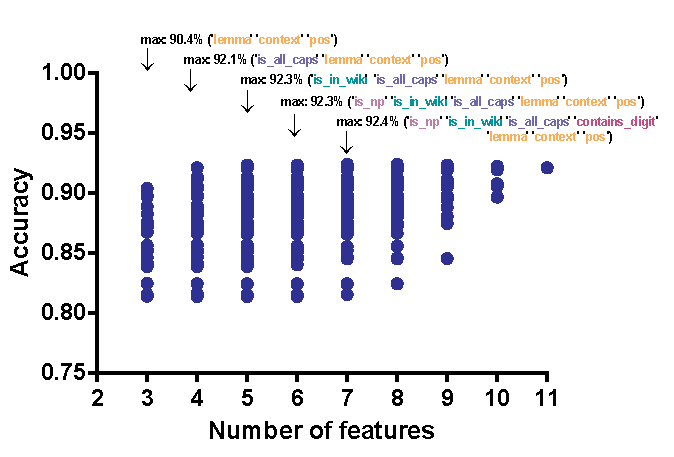
\includegraphics{accuracy.pdf}
			\caption{Accuracywerte der einzelnen Subsets. Jeder blaue Punkt stellt ein Subset dar.}
			\label{tab:accuracy}
		\end{figure}
		
		\begin{figure}[H]
			\centering
			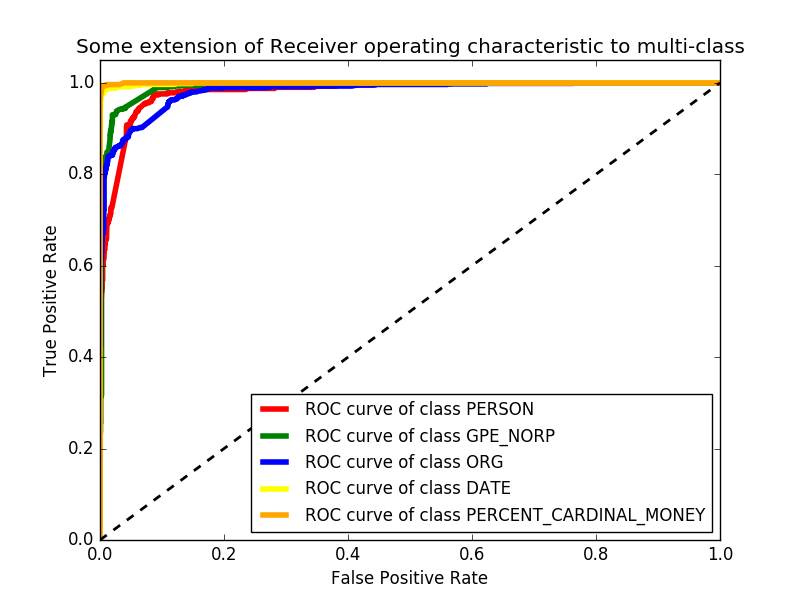
\includegraphics[scale=0.5]{roc_curve.png}
			\caption{ROC Kurve für das optimale Featureset mit sieben Features.}
			\label{tab:roc}
		\end{figure}
		

		
	\end{appendices}
		
\end{document}